%%%%%%%%%%%%%%%%%%%%%%%%%%%%%%%%%%%%%%%%%%%%%%%%%%%%%%%%%%%%%%%%%%%%%%%%%%%%%%%%
%%%
%%%  DATE CREATED:      2017-10-22
%%%
%%%  DATE LAST SAVED:   Time-stamp: <2017-10-23 20:17:20 (Mark.Wheldon)>
%%%
%%%  AUTHOR:            Mark Wheldon
%%%
%%%  PROJECT:           Bayesian Reconstruction
%%%
%%%  DESCRIPTION:
%%%
%%%  Slides for PopReconstrut demo to give after the talk on Bayesian
%%%  Reconstruction at Adrian R's workshop at IUSSP IPC 2017, Cape Town, South
%%%  Africa.
%%%
%%% ----------------------------------------------------------------------------
%%%
%%%  NOTES
%%%
%%%%%%%%%%%%%%%%%%%%%%%%%%%%%%%%%%%%%%%%%%%%%%%%%%%%%%%%%%%%%%%%%%%%%%%%%%%%%%%%


\documentclass[smaller,compress,table]{beamer}

\title[popReconstruct Demo]{popReconstruct Demonstration\\[-0.5em]\hspace*{-1em}\rule{1.2\paperwidth}{1pt}}
\subtitle{IUSSP International Population Conference, 2017}
\author{\large{Mark Wheldon}}
\institute{United Nations, Population Division\\and\\Auckland University of Technology, New Zealand}
\date{\scriptsize{
    \begin{tabular}{rp{0.7\textwidth}}
    \textbf{Acknowledgements:} & Joint work with Adrian Raftery, Sam Clark and Patrick Gerland\\
                           & NICHD, Grants R01~HD054511 and K01~HD057246 \\
                           & BayesPop Working Group, CSSS, and CSDE at the UW\\
                           & FHES at AUT\\[0.5em]
     \textbf{Disclaimer:}  & The views and opinions expressed in this presentation are those of the authors and do not necessarily represent those of the United Nations. This presentation has not been formally edited and cleared by the United Nations.
    \end{tabular}
    }}


%%% ----------------------------------------------------------------------------
%%% Std. Preamble
%%% ----------------------------------------------------------------------------

%%% ------------------------------------------------------------------
%%% LAYOUT, SPACING
%%% ------------------------------------------------------------------

%%%
%%% CHANGE DEFAULTS FOR BASIC SPACING, ALIGNMENT, SIZES, ETC.
%%%

%%
%% Spacing in and around figures
%%

%
% Reduce spacing above and below figures
%
\let\oldfigure\figure
\let\endoldfigure\endfigure
\renewenvironment{figure}%
{\begin{oldfigure}\vspace{-3ex}%
}%
{\end{oldfigure}\vspace{-3ex}%
}

%
% Captions
%
% \let\oldabovecaptionskip\abovecaptionskip
\addtolength{\abovecaptionskip}{-2ex}
\setbeamerfont{caption}{size=\scriptsize}


%%
%% Get line breaking in tt
%%

\newcommand*\justify{%
  \fontdimen2\font=0.4em% interword space
  \fontdimen3\font=0.2em% interword stretch
  \fontdimen4\font=0.1em% interword shrink
  \fontdimen7\font=0.1em% extra space
  \hyphenchar\font=`\-% allowing hyphenation
}%


%%%
%%% INSERT SECTION HEADER SLIDES
%%%

\newcommand{\sectiontitlepage}{%
\begin{frame}[plain]
\vfill
\begin{center}
\LARGE \bfseries \structure{
\insertsection}%
  \addtocounter{framenumber}{-1}
\end{center}
\vfill
\end{frame}
}

\newcommand{\subsectiontitlepage}{%
\begin{frame}[plain]
\vfill
\begin{center}
{\Large \itshape \structure{
\insertsubsection}%
}
  \addtocounter{framenumber}{-1}
\end{center}
\vfill
\end{frame}
}

\newcommand{\subsubsectiontitlepage}{%
\begin{frame}[plain]
\vfill
\begin{center}
{\large \structure{
\insertsubsubsection}%
}
  \addtocounter{framenumber}{-1}
\end{center}
\vfill
\end{frame}
}


%%% ------------------------------------------------------------------
%%% APPEARENCE TWEAKS
%%% ------------------------------------------------------------------

%%
%% Fonts
%%

\usepackage{lmodern}
\usepackage{fixmath}


%%
%% FOR SIMPLER FRAMETITLES
%%

\setbeamertemplate{frametitle}
{
\begin{centering}
\textbf{\usebeamercolor[bg]{frametitle} \insertframetitle}
\par
\end{centering}
}
\setbeamertemplate{headline}{%
\begin{beamercolorbox}[wd=\paperwidth,ht=2ex,dp=1ex,right]{}%
\end{beamercolorbox}}%

%%
%% COLOR THEMES
%%

\usecolortheme{whale}

%%
%% OUTER THEMES
%%

\setbeamertemplate{navigation symbols}{} % gets rid of navigation symbols
\setbeamertemplate{footline}{} % gets rid of bottom info lines
\setbeamertemplate{footline}{%
\begin{beamercolorbox}[wd=\paperwidth,ht=2.25ex,dp=1ex]{}%
  \color{gray}\hspace*{2ex}\insertsection\qquad \insertsubsection\qquad\insertsubsubsection\hfill\insertframenumber\hspace*{2ex}
\end{beamercolorbox}}           % PAGE NUMBERS W/O TOTAL PAGES

%%
%% INNER THEMES
%%

\useinnertheme{circles}

%%
%% NOTE PAGES
%%

\setbeamertemplate{note page}[compress]
\setbeamerfont{note page}{size=\footnotesize}
 \setbeameroption{show notes}
% \setbeameroption{show only notes}

%%
%% For Handouts
%%

\mode<handout>{%
  \usepackage{pgfpages}%
  \pgfpagesuselayout{4 on 1}[letterpaper,landscape,border shrink=5mm]%
  \setbeamercolor{background canvas}{bg=black!2}%
}

%%
%% OTHER OPTIONS
%%

\setbeamertemplate{frametitle continuation}[from second][ ] %no continuation numbers


%%% ------------------------------------------------------------------
%%% PDF SPECIFIC
%%% ------------------------------------------------------------------

%%%
%%% Frametitles in pdf bookmarks
%%%

% from: http://tex.stackexchange.com/questions/17230/beamer-how-to-make-each-frame-appear-in-the-pdf-toc

\usepackage{bookmark}
\usepackage{etoolbox}
\makeatletter
\apptocmd{\beamer@@frametitle}{
  \bookmark[page=\the\c@page,level=4]{#1}
  }%
  {\message{** patching of \string\beamer@@frametitle succeeded **}}%
  {\message{** patching of \string\beamer@@frametitle failed **}}%
\makeatother


%%% ------------------------------------------------------------------
%%% USEFUL PACAKGES
%%% ------------------------------------------------------------------

\usepackage{graphicx}
\usepackage{comment}
\usepackage{fancyvrb}
\usepackage{rotating}

%% Graphics extensions
\DeclareGraphicsExtensions{.png,.gif,.pdf}

%% XY pic
\usepackage{etex}
\usepackage[all]{xy}        % MUST load etex package as FIRST package

%% Tables
\usepackage{tabulary}
\usepackage{threeparttable}
\usepackage{colortbl}


%%% ------------------------------------------------------------------
%%% BIBLIOGRAPHY
%%% ------------------------------------------------------------------

% biblatex/biber seem to cause problems.

\usepackage[round]{natbib}


%%% ------------------------------------------------------------------
%%% NEW COMMANDS
%%% ------------------------------------------------------------------

%%%
%%% LISTS
%%%

% Itemize with labels
\newcommand\litem[1]{\item{\bfseries #1\enspace}}


%%%
%%% FORMATTING
%%%

% nowns (e.g., names of books, etc.)
\newcommand\Noun[1]{\emph{#1}}

% software packages
\newcommand\sware[1]{\emph{#1}}

%%%
%%% GRAPHICS WIDTHS
%%%

\newcommand{\GinTextwidth}{\setkeys{Gin}{keepaspectratio=true,width=\textwidth}}
\newcommand{\GinTextWidth}{\GinTextwidth}
\newcommand{\GinKARWid}[1]{\setkeys{Gin}{keepaspectratio=true,width=#1}}
\newcommand{\GinKARWidth}[1]{\setkeys{Gin}{keepaspectratio=true,width=#1}}


%%% ------------------------------------------------------------------
%%% NEW ENVIRONMENTS
%%% ------------------------------------------------------------------

%%
%% Additions
%%

\newenvironment{added}{\color{DodgerBlue4}}{}


%%% ------------------------------------------------------------------
%%% TEXT MACROS
%%% ------------------------------------------------------------------

%%%
%%% MATHS OPERATORS AND SYMBOLS
%%%

\usepackage{amsmath}

% Mathematical symbols
\newcommand{\norm}[1]{\lVert#1\rVert}
\newcommand{\cond}{\, \vert\, }
\newcommand{\ud}{\mathrm{d}}

\newcommand{\ci}{\perp\!\!\!\perp}
\newcommand\independent{\protect\mathpalette{\protect\independenT}{\perp}}
\def\independenT#1#2{\mathrel{\rlap{$#1#2$}\mkern2mu{#1#2}}}

%'_c_o_v_ariance _m_atrix
\newcommand{\cvm}{\makebox[0.38\width][l]{\ensuremath{\Sigma}}\raisebox{0.1\height}{\ensuremath{\vert}}}

% Vectors, matrices
\renewcommand{\vec}[1]{\boldsymbol{#1}}
\newcommand{\mat}[1]{\pmb{\mathrm{#1}}}

% Mathematical operators
\DeclareMathOperator{\logit}{logit}
\DeclareMathOperator{\diag}{diag}
\DeclareMathOperator{\odds}{odds}
\DeclareMathOperator{\Beta}{B}


% Statistical operators
\DeclareMathOperator{\E}{E}
\DeclareMathOperator{\var}{Var}
\DeclareMathOperator{\cor}{Cor}
\DeclareMathOperator{\cov}{Cov}
\DeclareMathOperator{\Var}{Var}
\DeclareMathOperator{\Cor}{Cor}
\DeclareMathOperator{\Cov}{Cov}
\DeclareMathOperator*{\median}{median}
% \DeclareMathOperator*{\mode}{mode}
\DeclareMathOperator*{\MAD}{MAD}
\DeclareMathOperator*{\MARE}{MARE}
\DeclareMathOperator*{\QAD}{QAD}

% Distributions
\DeclareMathOperator{\dUnif}{Unif}
\DeclareMathOperator{\dNorm}{Normal}
\DeclareMathOperator{\dMVNorm}{MVNormal}
\DeclareMathOperator{\dTruncNorm}{TruncNormal}
\DeclareMathOperator{\dLogistNorm}{LogisticNormal}
\DeclareMathOperator{\dExpo}{Expo}
\DeclareMathOperator{\dGamma}{Gamma}
\DeclareMathOperator{\dInvGamma}{InvGamma}
\DeclareMathOperator{\dLogNormal}{logNormal}
\DeclareMathOperator{\dBeta}{Beta}
\DeclareMathOperator{\dBin}{Bin}
\DeclareMathOperator{\dMult}{Mult}
\DeclareMathOperator{\dPois}{Pois}
\DeclareMathOperator{\dStudT}{{\it t\/}}


%%%
%%% DEMOGRAPHIC PARAMETERS
%%%

\newcommand{\ltp}[3]{{_#1}#2_#3}
\newcommand{\fertL}{{\kappa_L}}
\newcommand{\fertU}{{\kappa_U}}
\DeclareMathOperator{\TFR}{TFR}


%%%
%%% OTHER
%%%

% Possessive cite
\newcommand{\poscite}[1]{\citeauthor{#1}'s \citeyearpar{#1}}


% Question box
\newcommand{\alertbox}[2]{\fbox{\parbox{\textwidth}{\paragraph*{#1}#2}}}


%%% ------------------------------------------------------------------
%%% GLOSSARY
%%% ------------------------------------------------------------------

% \usepackage[sanitize=none,shortcuts,nonumberlist,numberedsection=autolabel,hyperfirst=false]{glossaries}
% \glsdisablehyper
% \renewcommand*{\glsautoprefix}{sec:glossary-}
% \loadglsentries{MCWLaTeXGlossary1.tex}
% \makeglossary

%% Language
\usepackage[american,newzealand]{babel}

% http://tex.stackexchange.com/questions/34921/how-to-overlap-images-in-a-beamer-slide
\def\Put(#1,#2)#3{\leavevmode\makebox(0,0){\put(#1,#2){#3}}}


% ---------------------------------------------------------------------------- %


\usepackage{Sweave}
\begin{document}
% ============================================================================ %

%%% ----------------------------------------------------------------------------
%%% Sweave Set Up
%%% ----------------------------------------------------------------------------

%% Graphics

\GinTextwidth

% Use:
% \GinSigPan (height = 7, width = 7),
% \GinSigPanLeg (height = 7, width = 7),
% \GinHalfPage (width=11,height=6.5),
% \GinFullPage (width=height=9)


%% Code

\DefineVerbatimEnvironment{Sinput}{Verbatim}{xleftmargin=2em}
\DefineVerbatimEnvironment{Soutput}{Verbatim}{xleftmargin=2em}
\DefineVerbatimEnvironment{Scode}{Verbatim}{xleftmargin=2em}
\fvset{listparameters={\setlength{\topsep}{0pt}}}
\renewenvironment{Schunk}{\vspace{\topsep}\scriptsize}{\vspace{\topsep}}

% ---------------------------------------------------------------------------- %



%++++++++++++++++++++++++++++++++++++++++++++++++++++++++++++++++++++++++++++++%

\begin{frame}[plain]
  \titlepage
  \addtocounter{framenumber}{-1}
\end{frame}


\begin{frame}
  \frametitle{Getting the Files}
  \begin{itemize}
  \item Create a directory on your hard drive to store the files.
  \item Go to \url{https://github.com/markalava/Bayesian-Reconstruction}
  \item Click ``Clone or download''.
  \item You can either download the \path{zip} file or `clone' the \sware{GitHub} repository.
  \item The repository contains the package as well as data files and \sware{R} scripts to reconstruct the population of Thailand.
  \end{itemize}
\end{frame}


\begin{frame}
  \frametitle{Getting the Files}
  \begin{center}
    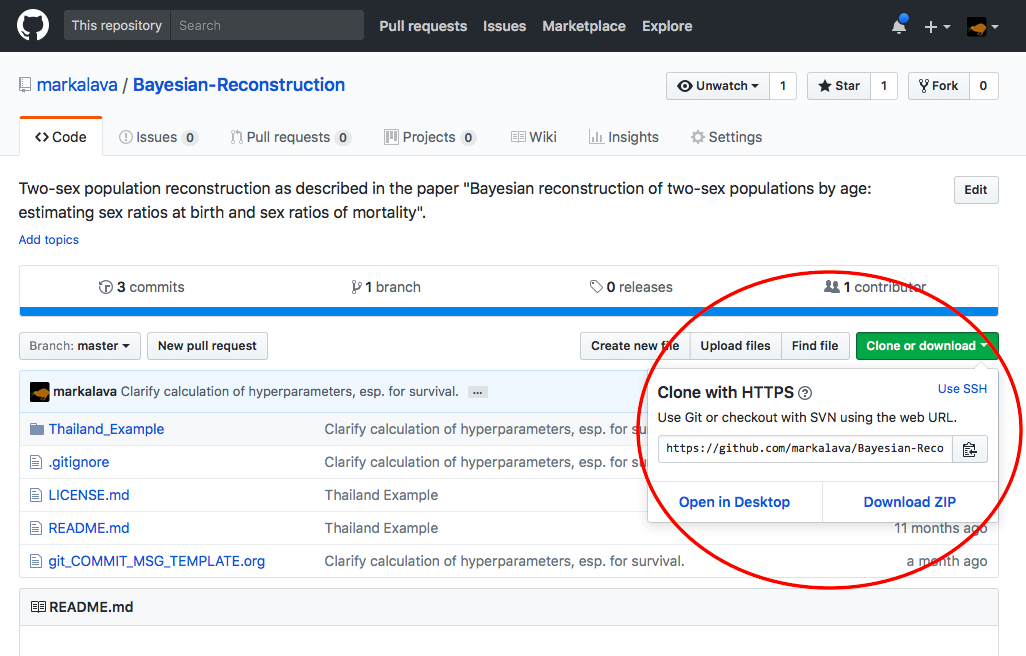
\includegraphics[width=\linewidth]{extras/github-bayesian-reconstruction.png}
  \end{center}
\end{frame}


\begin{frame}[fragile]
  \frametitle{Inputs}
  \begin{block}{Initial Estimates}
  \begin{itemize}
      \item The main inputs are initial estimates of fertility, migration, survival, population counts in the baseline year, population counts in subsequent years, and sex ratios at birth:
  \end{itemize}

\begin{Schunk}
\begin{Sinput}
> (load("../data/thai_initial_ests.RData"))
\end{Sinput}
\begin{Soutput}
[1] "asFertTHAI.mat"   "asMigTHAI.mat"    "asSurvTHAI.mat"   "baselineTHAI.mat"
[5] "censusTHAI.mat"   "srbTHAI.mat"     
\end{Soutput}
\end{Schunk}

  \end{block}

  \begin{block}{Separation Factors}
  \begin{itemize}
      \item Life table separation factors aid conversion among demographic parameters.
  \end{itemize}

\begin{Schunk}
\begin{Sinput}
> (load("../data/thai_sep_factors.RData"))
\end{Sinput}
\begin{Soutput}
[1] "thaiFemale.sf" "thaiMale.sf"  
\end{Soutput}
\end{Schunk}

  \end{block}
\end{frame}


\begin{frame}[fragile]
  \frametitle{Inputs}
  \begin{block}{Proposal Variances}
  \begin{itemize}
      \item Proposal variances are additional inputs that ensure efficient running of the MCMC algorithm.
      \item Tuning functions in \path{2_tuning.R} can be used to help select good values for these parameters.
  \end{itemize}

\begin{Schunk}
\begin{Sinput}
> (load("../data/thai_propvars.RData"))
\end{Sinput}
\begin{Soutput}
[1] "thai.propvar"
\end{Soutput}
\end{Schunk}

\end{block}
\end{frame}


\begin{frame}[fragile]
  \frametitle{Initial Estimates}
  \begin{block}{Fertility Rates and SRBs}
  \begin{itemize}
      \item Fertility rates and SRBs are matrices with five-year periods as columns, age-groups as rows.
  \end{itemize}

\begin{Schunk}
\begin{Sinput}
> asFertTHAI.mat[1:12, 1:5]
\end{Sinput}
\begin{Soutput}
         1960       1965       1970       1975        1980
0  0.00000000 0.00000000 0.00000000 0.00000000 0.000000000
5  0.00000000 0.00000000 0.00000000 0.00000000 0.000000000
10 0.00000000 0.00000000 0.00000000 0.00000000 0.000000000
15 0.05175459 0.06061538 0.06224863 0.06697348 0.056633004
20 0.24021806 0.23413036 0.22148542 0.21094695 0.163755256
25 0.28880806 0.27729894 0.24963584 0.19398416 0.154346419
30 0.27214926 0.25390511 0.21493142 0.15023581 0.103045913
35 0.21223853 0.19860950 0.16017444 0.10735185 0.060685573
40 0.11637142 0.12300785 0.09998354 0.05626398 0.041692712
45 0.02948599 0.03232336 0.02472358 0.02067992 0.008513132
50 0.00000000 0.00000000 0.00000000 0.00000000 0.000000000
55 0.00000000 0.00000000 0.00000000 0.00000000 0.000000000
\end{Soutput}
\end{Schunk}

\end{block}
\end{frame}


\begin{frame}[fragile]
  \frametitle{Initial Estimates}
  \begin{block}{Survival and Migration Proportions, Population Counts}
  \begin{itemize}
      \item The remaining inputs are lists of two components, ``female'' and ``male''.
      \item Each component is a matrix with five-year periods as columns, age-groups as rows.
  \end{itemize}

\begin{Schunk}
\begin{Sinput}
> lapply(asSurvTHAI.mat, "[", i = 1:3, j = 1:5)
\end{Sinput}
\begin{Soutput}
$female
        1960      1965      1970      1975      1980
0  0.9142663 0.9237345 0.9377636 0.9546893 0.9692136
5  0.9612171 0.9621474 0.9724710 0.9805215 0.9857410
10 0.9899652 0.9911082 0.9923885 0.9936778 0.9954615

$male
        1960      1965      1970      1975      1980
0  0.9108313 0.9224748 0.9340966 0.9461544 0.9605498
5  0.9611747 0.9639159 0.9731235 0.9801511 0.9830052
10 0.9881956 0.9895983 0.9911646 0.9926470 0.9943731
\end{Soutput}
\end{Schunk}

\end{block}
\end{frame}


\begin{frame}[fragile]
  \frametitle{Running the Reconstruction: \path{1_estimation.R}}
  \begin{itemize}
      \item Set-up

\begin{Schunk}
\begin{Sinput}
> set.seed(1)
> library(coda)
> data.path <- "data"
> prog.path <- "R_Code"
> results.path <- "results"
> if (!file.exists(results.path)) dir.create(results.path)
> example(source, echo = FALSE)
> sourceDir(prog.path)
\end{Sinput}
\begin{Soutput}
Calculate_Counts.R :
ccmp_femDom.R :
ChooseHyperparameters.R :
CondVariances.R :
EstModel_TwoSex.R :
Misc_Functions.R :
sampleFromPrior.R :
\end{Soutput}
\end{Schunk}


\end{itemize}
\end{frame}


\begin{frame}[fragile]
  \frametitle{Running the Reconstruction: \path{1_estimation.R}}
  \begin{itemize}
  \item Set the number of iterations.
\begin{Schunk}
\begin{Sinput}
> n.iter <- 17
> burn.in <- 3
\end{Sinput}
\end{Schunk}

  \item Convert elicited relative errors to hyperparameters.

\begin{Schunk}
\begin{Sinput}
> invGam.params <- make.hyper.params(absDev = list(fert = 0.1, 
+     surv = 0.1, mig = 0.2, pop = 0.1, srb = 0.1), prob = list(fert = 0.9, 
+     surv = 0.9, mig = 0.9, pop = 0.9, srb = 0.9), alpha = list(fert = 0.5, 
+     surv = 0.5, mig = 0.5, pop = 0.5, srb = 0.5), s.star = unlist(asSurvTHAI.mat))
> invGam.params[1:2]
\end{Sinput}
\begin{Soutput}
$al.f
[1] 0.5

$be.f
[1] 0.0001392358
\end{Soutput}
\end{Schunk}

  \end{itemize}
\end{frame}


\begin{frame}[fragile]
  \frametitle{Running the Reconstruction: \path{1_estimation.R}}
  \begin{itemize}
  \item Load proposal variances.


\begin{Schunk}
\begin{Sinput}
> withVisible(load(file = file.path("data", "thai_propvars.RData")))$value
\end{Sinput}
\begin{Soutput}
[1] "thai.propvar"
\end{Soutput}
\end{Schunk}


\item Set arguments
\begin{Schunk}
\begin{Sinput}
> estModArgs <- list(al.f = invGam.params$al.f, be.f = invGam.params$be.f,
+     al.s = invGam.params$al.s, be.s = invGam.params$be.s,
+     be.g = invGam.params$be.g, al.n = invGam.params$al.n,
+     al.srb = invGam.params$al.srb, be.srb = invGam.params$be.srb,
+     n.iter = n.iter, burn.in = burn.in,
+     start.f = asFertTHAI.mat, start.s = asSurvTHAI.mat,
+     start.b = baselineTHAI.mat, start.srb = srbTHAI.mat,
[..etc..]
\end{Sinput}
\end{Schunk}
  \item Run, then save the reconstruction.
\begin{Schunk}
  \begin{Sinput}
> ThaiMcmc <- do.call(popRecon.pop.est.sampler.aug07, args = estModArgs)
> save(ThaiMcmc, file = file.path(results.path, "thai_mcmc.RData"))
  \end{Sinput}
\end{Schunk}
  \end{itemize}
\end{frame}


\begin{frame}
  \frametitle{Tuning \path{2_tuning.R}}
  \begin{itemize}
  \item MCMC acceptance ratios can be examined to help find good proposal variances.
  \item Raftery-Lewis diagnostic can be run to help choose chain length.
  \end{itemize}
\end{frame}


\begin{frame}
  \frametitle{Proposal Variances}
  \begin{itemize}
  \item MCMC acceptance ratios between about 0.2 and 0.5 are acceptable.
  \item These can be plotted for each input parameter.
  \end{itemize}
  \begin{figure}
    \centering
    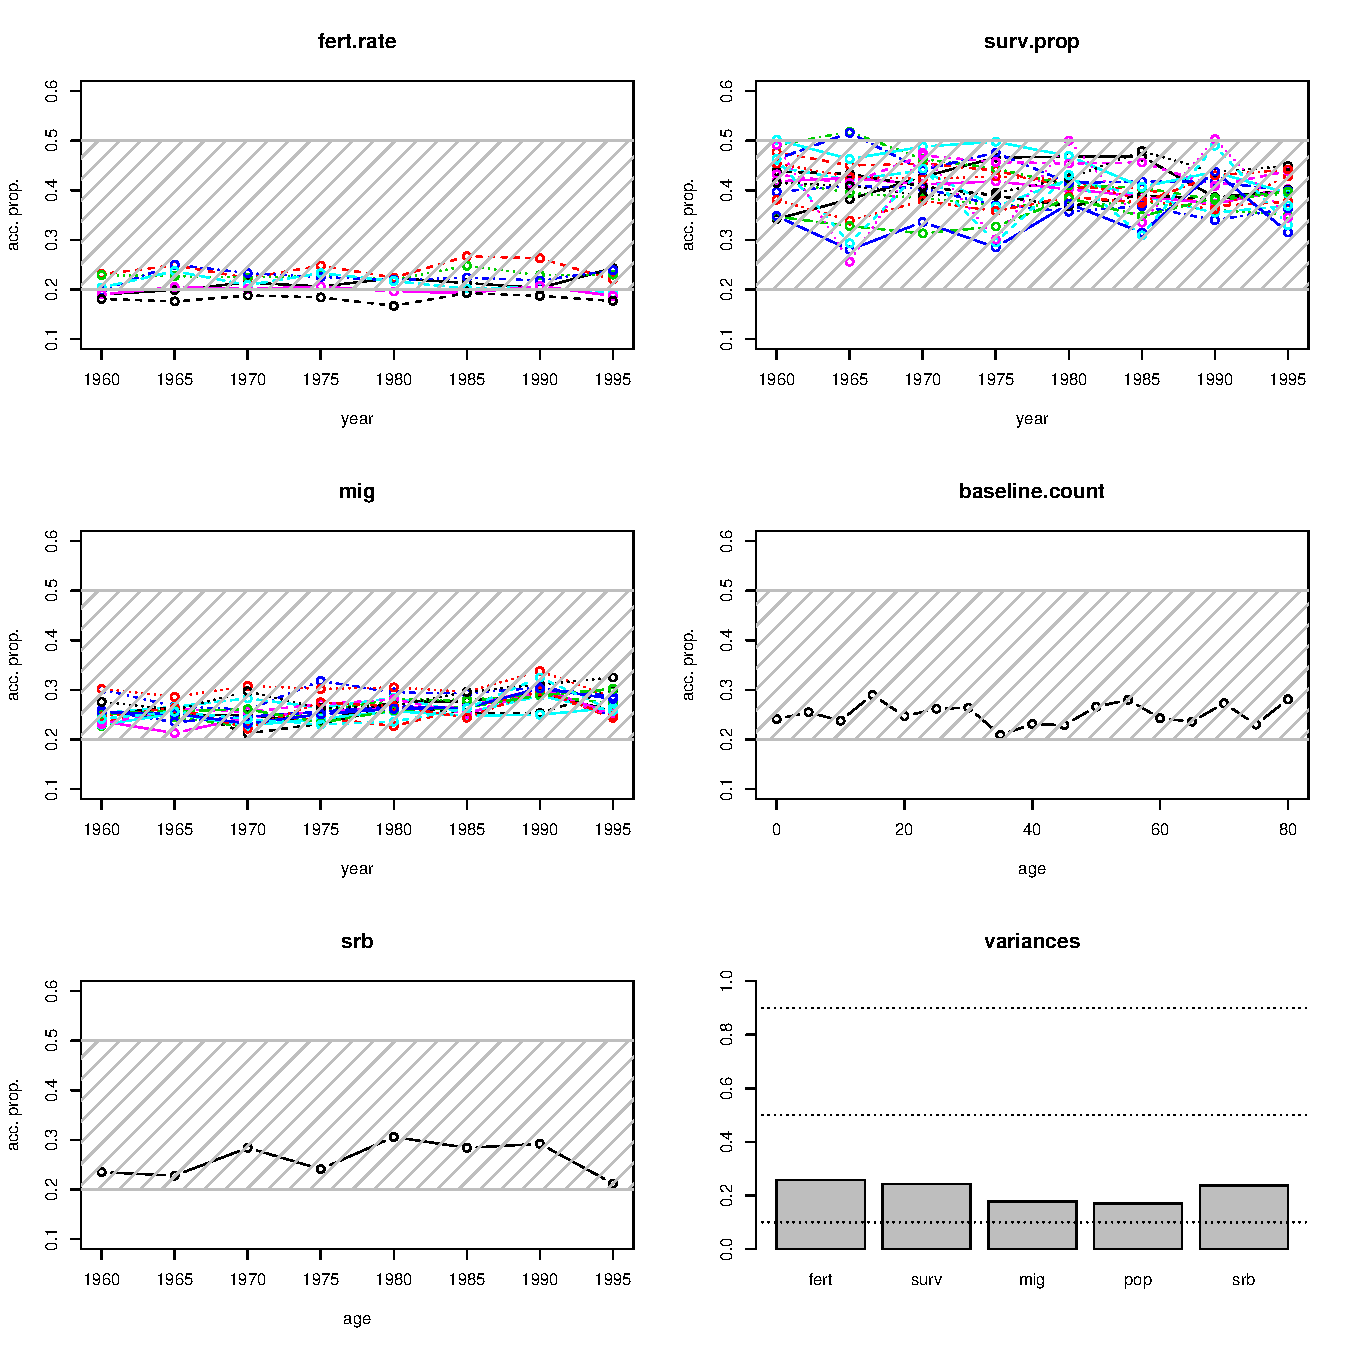
\includegraphics[width=0.8\linewidth,viewport=0 216 648 648,clip=true]{../results/Thai_20130612srb10_accProps.pdf}
    \caption{Metropolis acceptance ratios for fertility rate parameters. Example run with 1000 iterations and 1000 burn-in.}
  \end{figure}
\end{frame}


\begin{frame}[fragile]
  \frametitle{Proposal Variances}
  \begin{itemize}
  \item Automatic suggestions for proposal variances are generated if they need to be tuned.
  \item Finding good proposal variances is a matter of trial and error with short runs of the model.
  \end{itemize}
\begin{Schunk}
\begin{Sinput}
> vitalCondVars <- list()
> vitalCondVars$fert.rate <- chain.cond.vars.feb08(log(ThaiMcmc$fert.rate.mcmc))
> vitalCondVars$surv.prop <-
+     (chain.cond.vars.feb08(logit(ThaiMcmc$surv.prop.mcmc[["female"]])) +
+     chain.cond.vars.feb08(logit(ThaiMcmc$surv.prop.mcmc[["male"]])))/2
\end{Sinput}
\end{Schunk}
\end{frame}


\begin{frame}
  \frametitle{Sample from the Prior Distribution \path{2_sample_from_prior.R}}
  \begin{itemize}
  \item To be able to create plots that compare the prior and posterior distributions, run \path{2_sample_from_prior.R}.
  \item Note: this can take a long time.
  \end{itemize}
\end{frame}


\begin{frame}[fragile]
  \frametitle{Post Process \path{3_post_process.R}}
  \begin{itemize}
  \item Output from \path{1_estimation.R} needs to be post-processed (e.g., to convert rates to counts).
  \end{itemize}
\begin{Schunk}
\begin{Sinput}

### Calculate Counts from Posterior

> nF <- ncol(ThaiMcmc$fixed.params$mean.mig.prop$female) *
+    nrow(ThaiMcmc$fixed.params$mean.mig.prop$female)

> proj.to.counts.aug22(fert.rate.mcmc = ThaiMcmc$fert.rate.mcmc
+                     ,surv.prop.mcmc = list(female = ThaiMcmc$surv.prop.mcmc$female
+                      ,male = ThaiMcmc$surv.prop.mcmc$male)
+                     ,mig.prop.mcmc = list(female = ThaiMcmc$mig.prop.mcmc$female
+                      ,male = ThaiMcmc$mig.prop.mcmc$male)
+                     ,baseline.count.mcmc = list(female =
+                      ,male = ThaiMcmc$baseline.count.mcmc$male)
+                     ,pop.count.mcmc = list(female = ThaiMcmc$lx.mcmc$female
+                      ,male = ThaiMcmc$lx.mcmc$male)
+                     ,sep.factors = list(female = thaiFemale.sf[1:nF]
+                      ,male = thaiMale.sf[1:nF])
+                     ,srb.mcmc = ThaiMcmc$srb.mcmc
+                     ,name.pref = "Thai."
+                     ,name.suf = ""
+                     ,file.backed = TRUE
+                     ,ccmp.f = "ccmp.femDom.jun12"
+                     )
[..etc..]
\end{Sinput}
\end{Schunk}
\end{frame}


\begin{frame}
  \frametitle{Plot Results \path{4_plots_results.R}}
  \begin{itemize}
    \item To plot some results, use the functions and calls in \path{4_plots_results.R}.
  \end{itemize}
  \begin{figure}
    \centering    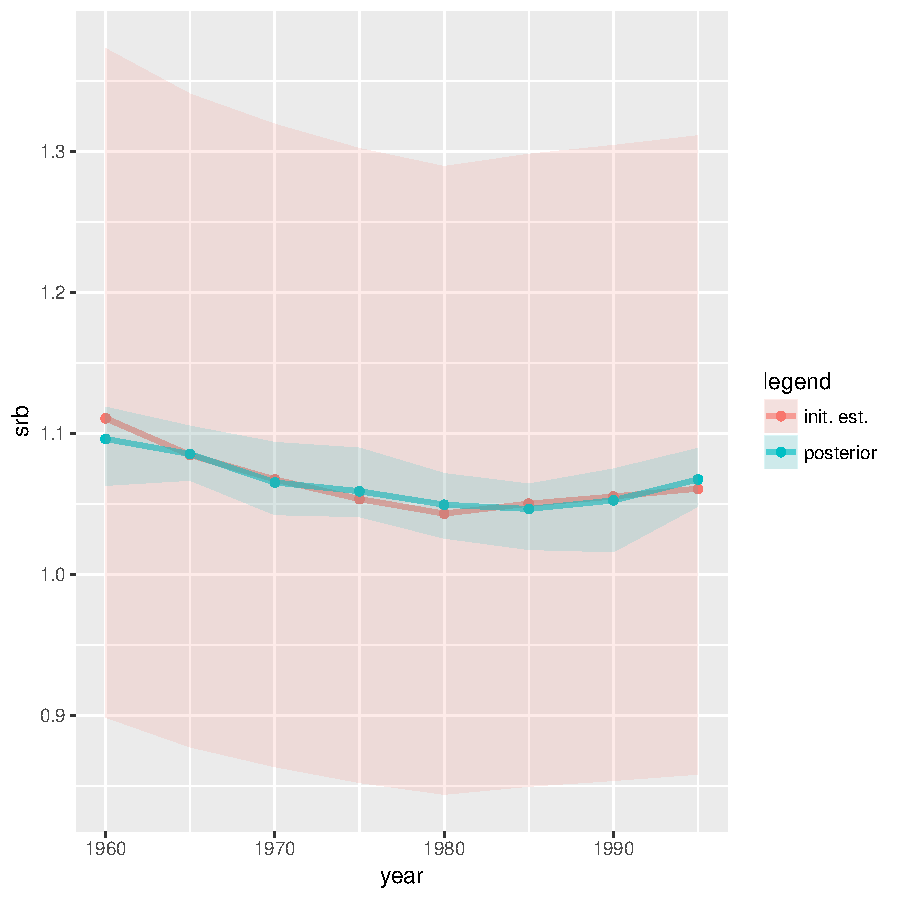
\includegraphics[width=0.5\textwidth]{extras/Thai_srb_priorpost_q95_iussp2017_slides.pdf}
    \caption{Sex ratio at birth. Prior (red) and posterior (blue) 95\% credible intervals and prior and posterior medians.}
  \end{figure}
\end{frame}



% ++++++++++++++++++++++++++++++++++++++++++++++++++++++++++++++++++++++++++++ %

%\appendix

%% \section{References}
%% \sectiontitlepage

%% \begin{frame}[allowframebreaks,plain]
%%   \scriptsize
%%   \bibliographystyle{asa}
%%   \def\newblock{}
%%   \bibliography{PPGpRefs}
%% \end{frame}


%% \section{Additional Material}




% ============================================================================ %
\end{document}
